\documentclass{article}

\usepackage[letterpaper, margin=1in]{geometry}
\usepackage{hyperref}
\usepackage{fontspec}
\usepackage{graphicx}
\usepackage{wrapfig}

\setmainfont{Arial}
\pagestyle{empty}

\title{Currículum Vitae}
\author{Fabián Eduardo Ferrada Merino}
\date{18 de Mayo, 2026}
\begin{document}
	\begin{wrapfigure}[8]{l}{0.18\textwidth}
		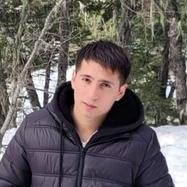
\includegraphics[width=0.18\textwidth]{foto.jpg}
	\end{wrapfigure}

	\Large \textbf{Fabián Eduardo Ferrada Merino} \\
	
	\normalsize
	Contacto: \url{mferradafabian@gmail.com}

	Celular: +56 9 7920 1926
	
	Ciudad: Chillán, Ñuble
	
	GitHub: https://github.com/fferradamerino
	
	Linkedin: https://linkedin.com/in/fabián-ferrada-merino \\
	
	\noindent
	\textbf{Resumen profesional}
	
	Ingeniero Civil en Informática enfocado en desarrollo backend y sistemas de bajo nivel (Spring Boot, PostgreSQL, Go, Python). Como docente universitario he desarrollado una serie de herramientas y materiales de enseñanza, fortaleciendo mi comprensión técnica integral y mi capacidad para comunicar conceptos complejos. \\
	
	\noindent
	\textbf{Experiencia Laboral}
	
	\textit{\textbf{Desarrollador de Realidad Extendida con Unity (Chillán, Ñuble)}} [Jornada parcial -- Presencial] \par
	Septiembre, 2026 --- Actualidad \par
	- Construcción de una simulación de XR para la capacitación de personal de bomberos. \par
	- Participo dentro de un equipo multidisciplinario que involucra inteligencia artificial y desarrollo backend. \par
	- Actualmente he logrado implementar un 60\% del proyecto propuesto. \\
	
	\textit{\textbf{Docente en Universidad del Bío-Bío (Chillán, Ñuble)}} [Jornada parcial -- Presencial] \par
	Marzo, 2026 --- Actualidad \par
	- Desarrollé un simulador de software de arquitectura RISC para la enseñanza de sistemas de bajo nivel. \par
	- Logré la adopción activa del simulador por más de 40 estudiantes para la validación de su diseño. \par
	- Actualmente trabajo en el desarrollo de herramientas y material de estudio en la asignatura de Computación Gráfica y Realidad Extendida. \\
	
	\textit{\textbf{Practicante Universitario en Vita Wines House (Chillán, Ñuble)}} [Jornada completa -- Híbrido] \par
	Diciembre, 2024 --- Febrero, 2025 \par
	- Construí pipelines de datos eficientes para el procesamiento y entrenamiento de modelos de IA. \par
	- Desarrollé un prototipo interactivo en Godot con chatbot y avatar virtual, integrando la API REST de Hugging Face. \par
	- Aceleré la validación técnica del producto, superando los objetivos globales del proyecto en un 25\% de forma anticipada. \\
	
	\textit{\textbf{Ayudante Universitario en U. del Bío-Bío (Chillán, Ñuble)}} [Jornada parcial -- Presencial] \par
	Septiembre, 2024 --- Diciembre, 2024 \par
	- Elaboré material técnico y código de ejemplo sobre algoritmos y lógica matemática para más de 50 estudiantes. \par
	- Realicé code-reviews y evaluaciones, simplificando la explicación de conceptos técnicos complejos. \\
	
	\textit{\textbf{Desarrollador Backend en Equipo Ntek (Chillán, Ñuble)}} [Jornada parcial -- Híbrido] \par
	Abril, 2024 --- Mayo, 2024 \par
	- Diseñé y desarrollé APIs robustas en Scala con bases de datos PostgreSQL para soportar el core del producto. \par
	- Traduje requerimientos de negocio en soluciones técnicas, levantando feedback iterativo con más de 5 clientes. \\
	
	\textit{\textbf{Practicante Universitario en Corfo (Chillán, Ñuble)}} [Jornada completa -- Remoto] \par
	Enero, 2024 --- Marzo, 2024 \par
	- Desarrollé la arquitectura backend y gestión de datos de una app móvil para PyMEs durante todo su ciclo de vida. \par
	- Optimicé las funcionalidades del sistema aplicando la retroalimentación obtenida directamente de clientes clave. \par
	- Alcancé un 90\% de completitud del proyecto, entregando una base de código sólida y preparada para producción. \\
	
	\noindent
	\textbf{Proyectos}

	\textit{\textbf{Sistema municipal de Postulación de Becas}} \par
	Periodo: Enero, 2025 -- Actualidad \par
	Tecnologías: Spring Boot, Spring Security, Angular, MySQL, Docker y Nginx. \par
	Enlace: github.com/fferradamerino/sistemabecas \par
	Desarrollo de una plataforma web moderna y eficiente para la gestión de becas, dirigida a postulantes y administradores. Fue construida con Spring Boot y Angular, integrando diseño de base de datos (ER), orquestación con Docker y un proxy inverso (Nginx) para optimizar la seguridad. \\
	
	\textit{\textbf{Diseño, Implementación y Simulación de la Arquitectura de Microprocesador M32 en Logisim Evolution (Universidad del Bío-Bío) [Proyecto de tesis]}} \par
	Periodo: Mayo, 2025 -- Enero, 2026 \par
	Tecnologías: Logisim Evolution, Python, Java, Mockito + JUnit, y GitHub \par Actions. \par
	Enlace: github.com/fferradamerino/m32logievo \par
	Implementación de la arquitectura M32 utilizando Logisim Evolution y técnicas de microprogramación. Actualmente utilizado por la asignatura de Arquitectura de Computadores en la Universidad del Bío-Bío. \\
	
	\textit{\textbf{BND Extract}} \par
	Periodo: Octubre, 2025 -- Noviembre, 2025 \par
	Tecnologías: Go y Ghidra (framework de ingeniería inversa). \par
	Enlace: github.com/fferradamerino/bnd\_extract \par
	Herramienta desarrollada a través de un proyecto de ingeniería inversa sobre el código del videojuego Kuon (2004) con el fin de hacer modificaciones (modding) de assets en dicho videojuego. \\
	
	\textit{\textbf{Generador cuántico de números aleatorios (simulado con Qiskit)}} \par
	Periodo: Septiembre, 2025 \par
	Tecnologías: Python y Qiskit. \par
	Enlace: github.com/fferradamerino/generador\_aleatorio\_cuantico \par
	Desarrollado utilizando Python y Qiskit, fue concebido como un proyecto experimental durante una charla de computación cuántica realizada en la Universidad del Bío-Bío. \\
	
	\textit{\textbf{Biblioteca de carga de archivos PNG}} \par
	Periodo: Enero, 2024 -- Marzo, 2024 \par
	Tecnologías: Go. \par
	Enlace: github.com/fferradamerino/pngloader \par
	Desarrollado como una investigación personal sobre el formato de imágenes PNG. Su propósito fue la carga de texturas en un proyecto de \textit{game engine} utilizando Go y OpenGL. \\
	
	\noindent
	\textbf{Habilidades, herramientas y lenguajes de programación}

	\begin{itemize}
		\item Lenguajes de programación: Java, Python, TypeScript, SQL, Scala, HTML, Assembler y Go.
		\item Frameworks y Librerías: Angular, Spring (Boot y Security), ReactJS, React Native y JUnit.
		\item Herramientas de software: Nginx, Docker, Linux, Google Cloud Platform y PostgreSQL.
		\item Habilidades: Desarrollo Backend, IA, Internet de las Cosas y Computación Gráfica.
		\item Idiomas: Español e Inglés Profesional.
	\end{itemize}
	
	\noindent
	\textbf{Educación}
	
	Universidad del Bío-Bío --- Ingeniería Civil en Informática \par
	Marzo, 2020 --- Marzo, 2026 \\
	
	\noindent
	\textbf{Certificaciones}: Canva para Eduación Creación y diseño de recursos didácticos [Universidad del Bío-Bío, 2026]; Domina la IA con Gemini [Santander Academy, 2026]; Certificate for Claude Code in Action [Anthropic, 2026]; Certificación en Gestión Ágil de Proyectos [Servicio Civil de Chile, 2026]; Learn React [Codecademy, 2025]; Quantum Computing Made Simple [Udemy, 2025]
	
\end{document}